% Options for packages loaded elsewhere
\PassOptionsToPackage{unicode}{hyperref}
\PassOptionsToPackage{hyphens}{url}
%
\documentclass[
  ,man]{apa6}
\usepackage{amsmath,amssymb}
\usepackage{iftex}
\ifPDFTeX
  \usepackage[T1]{fontenc}
  \usepackage[utf8]{inputenc}
  \usepackage{textcomp} % provide euro and other symbols
\else % if luatex or xetex
  \usepackage{unicode-math} % this also loads fontspec
  \defaultfontfeatures{Scale=MatchLowercase}
  \defaultfontfeatures[\rmfamily]{Ligatures=TeX,Scale=1}
\fi
\usepackage{lmodern}
\ifPDFTeX\else
  % xetex/luatex font selection
\fi
% Use upquote if available, for straight quotes in verbatim environments
\IfFileExists{upquote.sty}{\usepackage{upquote}}{}
\IfFileExists{microtype.sty}{% use microtype if available
  \usepackage[]{microtype}
  \UseMicrotypeSet[protrusion]{basicmath} % disable protrusion for tt fonts
}{}
\makeatletter
\@ifundefined{KOMAClassName}{% if non-KOMA class
  \IfFileExists{parskip.sty}{%
    \usepackage{parskip}
  }{% else
    \setlength{\parindent}{0pt}
    \setlength{\parskip}{6pt plus 2pt minus 1pt}}
}{% if KOMA class
  \KOMAoptions{parskip=half}}
\makeatother
\usepackage{xcolor}
\usepackage{graphicx}
\makeatletter
\def\maxwidth{\ifdim\Gin@nat@width>\linewidth\linewidth\else\Gin@nat@width\fi}
\def\maxheight{\ifdim\Gin@nat@height>\textheight\textheight\else\Gin@nat@height\fi}
\makeatother
% Scale images if necessary, so that they will not overflow the page
% margins by default, and it is still possible to overwrite the defaults
% using explicit options in \includegraphics[width, height, ...]{}
\setkeys{Gin}{width=\maxwidth,height=\maxheight,keepaspectratio}
% Set default figure placement to htbp
\makeatletter
\def\fps@figure{htbp}
\makeatother
\setlength{\emergencystretch}{3em} % prevent overfull lines
\providecommand{\tightlist}{%
  \setlength{\itemsep}{0pt}\setlength{\parskip}{0pt}}
\setcounter{secnumdepth}{-\maxdimen} % remove section numbering
% Make \paragraph and \subparagraph free-standing
\ifx\paragraph\undefined\else
  \let\oldparagraph\paragraph
  \renewcommand{\paragraph}[1]{\oldparagraph{#1}\mbox{}}
\fi
\ifx\subparagraph\undefined\else
  \let\oldsubparagraph\subparagraph
  \renewcommand{\subparagraph}[1]{\oldsubparagraph{#1}\mbox{}}
\fi
\newlength{\cslhangindent}
\setlength{\cslhangindent}{1.5em}
\newlength{\csllabelwidth}
\setlength{\csllabelwidth}{3em}
\newlength{\cslentryspacingunit} % times entry-spacing
\setlength{\cslentryspacingunit}{\parskip}
\newenvironment{CSLReferences}[2] % #1 hanging-ident, #2 entry spacing
 {% don't indent paragraphs
  \setlength{\parindent}{0pt}
  % turn on hanging indent if param 1 is 1
  \ifodd #1
  \let\oldpar\par
  \def\par{\hangindent=\cslhangindent\oldpar}
  \fi
  % set entry spacing
  \setlength{\parskip}{#2\cslentryspacingunit}
 }%
 {}
\usepackage{calc}
\newcommand{\CSLBlock}[1]{#1\hfill\break}
\newcommand{\CSLLeftMargin}[1]{\parbox[t]{\csllabelwidth}{#1}}
\newcommand{\CSLRightInline}[1]{\parbox[t]{\linewidth - \csllabelwidth}{#1}\break}
\newcommand{\CSLIndent}[1]{\hspace{\cslhangindent}#1}
\ifLuaTeX
\usepackage[bidi=basic]{babel}
\else
\usepackage[bidi=default]{babel}
\fi
\babelprovide[main,import]{english}
% get rid of language-specific shorthands (see #6817):
\let\LanguageShortHands\languageshorthands
\def\languageshorthands#1{}
% Manuscript styling
\usepackage{upgreek}
\captionsetup{font=singlespacing,justification=justified}

% Table formatting
\usepackage{longtable}
\usepackage{lscape}
% \usepackage[counterclockwise]{rotating}   % Landscape page setup for large tables
\usepackage{multirow}		% Table styling
\usepackage{tabularx}		% Control Column width
\usepackage[flushleft]{threeparttable}	% Allows for three part tables with a specified notes section
\usepackage{threeparttablex}            % Lets threeparttable work with longtable

% Create new environments so endfloat can handle them
% \newenvironment{ltable}
%   {\begin{landscape}\centering\begin{threeparttable}}
%   {\end{threeparttable}\end{landscape}}
\newenvironment{lltable}{\begin{landscape}\centering\begin{ThreePartTable}}{\end{ThreePartTable}\end{landscape}}

% Enables adjusting longtable caption width to table width
% Solution found at http://golatex.de/longtable-mit-caption-so-breit-wie-die-tabelle-t15767.html
\makeatletter
\newcommand\LastLTentrywidth{1em}
\newlength\longtablewidth
\setlength{\longtablewidth}{1in}
\newcommand{\getlongtablewidth}{\begingroup \ifcsname LT@\roman{LT@tables}\endcsname \global\longtablewidth=0pt \renewcommand{\LT@entry}[2]{\global\advance\longtablewidth by ##2\relax\gdef\LastLTentrywidth{##2}}\@nameuse{LT@\roman{LT@tables}} \fi \endgroup}

% \setlength{\parindent}{0.5in}
% \setlength{\parskip}{0pt plus 0pt minus 0pt}

% Overwrite redefinition of paragraph and subparagraph by the default LaTeX template
% See https://github.com/crsh/papaja/issues/292
\makeatletter
\renewcommand{\paragraph}{\@startsection{paragraph}{4}{\parindent}%
  {0\baselineskip \@plus 0.2ex \@minus 0.2ex}%
  {-1em}%
  {\normalfont\normalsize\bfseries\itshape\typesectitle}}

\renewcommand{\subparagraph}[1]{\@startsection{subparagraph}{5}{1em}%
  {0\baselineskip \@plus 0.2ex \@minus 0.2ex}%
  {-\z@\relax}%
  {\normalfont\normalsize\itshape\hspace{\parindent}{#1}\textit{\addperi}}{\relax}}
\makeatother

% \usepackage{etoolbox}
\makeatletter
\patchcmd{\HyOrg@maketitle}
  {\section{\normalfont\normalsize\abstractname}}
  {\section*{\normalfont\normalsize\abstractname}}
  {}{\typeout{Failed to patch abstract.}}
\patchcmd{\HyOrg@maketitle}
  {\section{\protect\normalfont{\@title}}}
  {\section*{\protect\normalfont{\@title}}}
  {}{\typeout{Failed to patch title.}}
\makeatother

\usepackage{xpatch}
\makeatletter
\xapptocmd\appendix
  {\xapptocmd\section
    {\addcontentsline{toc}{section}{\appendixname\ifoneappendix\else~\theappendix\fi\\: #1}}
    {}{\InnerPatchFailed}%
  }
{}{\PatchFailed}
\keywords{Backwards Masking, Temporal Integration, Vision, Individual Differences}
\DeclareDelayedFloatFlavor{ThreePartTable}{table}
\DeclareDelayedFloatFlavor{lltable}{table}
\DeclareDelayedFloatFlavor*{longtable}{table}
\makeatletter
\renewcommand{\efloat@iwrite}[1]{\immediate\expandafter\protected@write\csname efloat@post#1\endcsname{}}
\makeatother
\usepackage{csquotes}
\usepackage{bm}
\usepackage{amsmath}
\usepackage{setspace}
\usepackage{pcl}
\ifLuaTeX
  \usepackage{selnolig}  % disable illegal ligatures
\fi
\IfFileExists{bookmark.sty}{\usepackage{bookmark}}{\usepackage{hyperref}}
\IfFileExists{xurl.sty}{\usepackage{xurl}}{} % add URL line breaks if available
\urlstyle{same}
\hypersetup{
  pdftitle={Individual Differences In Perception Do Not Reflect Temporal Integration in A Perceptual Moment},
  pdfauthor={Aaron E. Fawcett1, Mahbod Mehrvarz1, \& Jeffrey N. Rouder1},
  pdflang={en-EN},
  pdfkeywords={Backwards Masking, Temporal Integration, Vision, Individual Differences},
  hidelinks,
  pdfcreator={LaTeX via pandoc}}

\title{Individual Differences In Perception Do Not Reflect Temporal Integration in A Perceptual Moment}
\author{Aaron E. Fawcett\textsuperscript{1}, Mahbod Mehrvarz\textsuperscript{1}, \& Jeffrey N. Rouder\textsuperscript{1}}
\date{}


\shorttitle{Individual Differences In Perception}

\authornote{

Version 1, Aug, 2024. AEF was supported by a Undergraduate Research Opportunity Grant from the University of California, Irvine and by NSF 2126976. JNR was supported by ONR N00014-23-1-2792.\\
Open Science Practices: The data, analysis scripts, and code used to generate the figures are openly available at \url{https://github.com/specl/ind-permom}.

Correspondence concerning this article should be addressed to Jeffrey N. Rouder, Department of Cognitive Science, University of California, Irvine, CA, 92697. E-mail: \href{mailto:jrouder@uci.edu}{\nolinkurl{jrouder@uci.edu}}

}

\affiliation{\vspace{0.5cm}\textsuperscript{1} University of California, Irvine}

\abstract{%
Stimulus duration has the opposite effect in masking and fusion tasks: longer durations enhance performance in masking tasks but impair it in fusion tasks.Several visual theories explain these and related phenomena with recourse to small temporal window where stimuli are integrated or superimposed. Accordingly, individuals with a long temporal window should exibit good performance in the fusion task and poor performance in the masking task. Therefore, performance in these two tasks should result in a negative correlation. We tested this negative correlation and found decisive evidence to the contrary, a positive correlation (\(N=21\), \(BF=256\)). People who perform well on the fusion task also perform well on the masking task. Hence, individual variation in a temporal window does not drive individual differences in vision. Instead, we suspect the positive correlation reflects a common ability to read out from and to refresh iconic storage.
}



\begin{document}
\maketitle

Consider two visual paradigms where time or duration plays an opposing role. One of these two is \emph{backwards masking}, and an example is shown in Figure \ref{fig:paradigm}A. A typical backwards-masking paradigm goes as follows: First, a target stimulus, a single dot in the figure, is briefly flashed. Then, after a delay, it is subsequently masked, which is composed of an array of dots. The delay between the target and mask is called the \emph{interstimulus interval} (ISI), and the duration of the ISI is critical. If the duration is long, then the target is easily seen; if it is short, then the target is not as easily seen. In fact, in most backwards masking paradigms, visibility rises monotonically with ISI duration (Breitmeyer, 1984).

\begin{figure}[h]
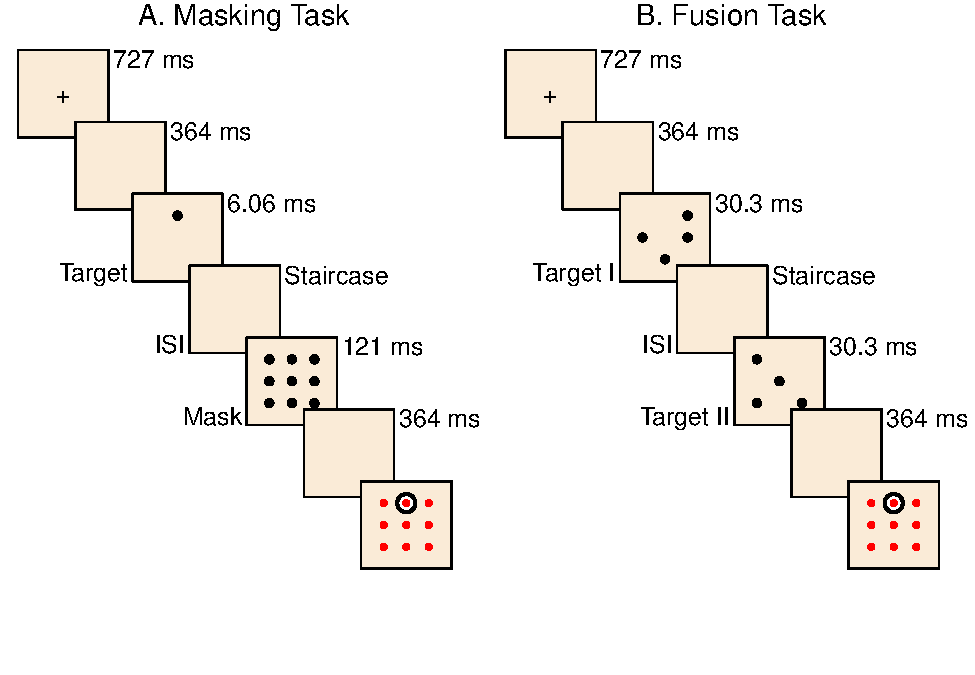
\includegraphics{p_files/figure-latex/paradigm-1} \caption{The trial structure of the two tasks used in the experiment. The 3-by-3 grid is illustrative; in the experiment the grid was 5-by-5 in size.}\label{fig:paradigm}
\end{figure}

Duration plays an opposite role in \emph{fusion} tasks. A classic fusion task, from Di Lollo and Wilson (1978), is shown in Figure \ref{fig:paradigm}B. Here, participants are shown two temporally separated targets. In this case, each target is 4 of 9 dots. If the targets are presented simultaneously, then the missing dot is obvious. As the duration between the targets is lengthened, performance suffers.

The opposing role of duration in these two paradigms is not surprising. One simple explanation is that performance is mediated by integration of visual-stimulus events in a brief temporal window of about 100 ms. Events that fall within the temporal window are bound together into one percept; those that are outside of it are differentiated into separate percepts. The window has been called the perceptual moment (Stroud, 1956), and the motif that there is a small temporal integration window is common in theories of vision and masking (Allport, 1968; Busey \& Loftus, 1994; Di Lollo, 1980; Kahneman, 1968; Scharnowski, Hermens, \& Herzog, 2007; Smith, 1995). If two stimuli are in the window, then they are superimposed resulting in better performance in the fusion task. By the same token, this superposition results in worse performance in the masking task as the mask obscures the target. And, accordingly, if an individual has a long temporal window, then they should be relatively good at the fusion task at the expense of the masking task and, conversely, if they have a short temporal window, then they should be relatively good at the masking task at the expense of the fusion task.

This converse relationship gives rise to a novel prediction about individual differences. If variability in the time frame of temporal integration is a salient individual-difference factor in perception, then there should be a negative correlation. In other words, individuals who are relatively better in one of two task should be relatively worse in the other. This converse relationship, should it exist, is novel precisely because such negative correlations are rarely if ever observed in measures of cognitive performance. People who are good at one task tend to be good at other tasks. This positive correlation is almost always observed and known as Spearman's positive manifold (Ritchie, 2015).

The main question here is whether performance across masking and fusion tasks is negatively correlated, in concordance with substantial variability in the temporal window, or positively correlated, in concordance with the positive manifold. The following experiment is an individual-differences study where individuals alternated between the two tasks. To foreshadow, the results are definitive---there is a positive correlation in performance. People who need relatively small ISIs in the backwards masking task can still integrate over relatively large ISIs in the fusion task.

\hypertarget{method}{%
\section{Method}\label{method}}

\hypertarget{irb}{%
\subsection{IRB}\label{irb}}

The experiment was run in accordance with UCI IRB 2823, self-determined exempt (Category 3) with a waiver from obtaining written documentation of informed consent.

\hypertarget{participants}{%
\subsection{Participants}\label{participants}}

Twenty-one University of California-Irvine undergraduate students served as participants in exchange for extra credit in an introductory psychology course. Participants were enrolled into an optional-sampling strategy until the Bayes factor exceeded 10-to-1 in favor of positive or negative correlation, with a bottom threshold of 20 participants (Schönbrodt, Wagenmakers, Zehetleitner, \& Perugini, 2017).

\hypertarget{tasks-apparatus}{%
\subsection{Tasks \& Apparatus}\label{tasks-apparatus}}

The experiment was comprised of two tasks: a masking task and a fusion task. In both tasks, the screen resolution was set at 1920 pixels \(\times\) 1080 pixels, and the screen refresh rate was set at 165hz. The screen measured 52.6 cm \(\times\) 29.6 cm with each pixel measuring .0274 cm on a side. Participants sat 176 cm from the screen.

\hypertarget{masking-task.}{%
\subsubsection{Masking Task.}\label{masking-task.}}

The basic structure of the masking task is shown in Figure \ref{fig:paradigm}A. The grid used was a 5-by-5 (25 element) grid similar to the 3-by-3 grid shown in Figure \ref{fig:paradigm}. This grid was 192 pixels on a side and subtended 1.7 degrees of visual angle. The background was black, and stimuli and masks were drawn in white. First, participants were presented with a fixation cross (727.3 ms) followed by a blank (363.6 ms). The target, a single white dot whose location was randomly selected from one of 16 positions in the interior of the five-by-five grid, was displayed next for 6.06 ms (1 refresh at 165hz). This target was followed by a blank interstimulus interval (ISI), the duration was determined by an adaptive staircase, discussed subsequently, so that performance was intermediate between floor and ceiling. A subsequent mask, consisting of an array of 25 white dots arranged in a 5 x 5 grid, was then displayed for 121.2 ms. The mask was followed by a blank (363.6 ms) and a response screen, which was comprised of smaller red dots. The participant then moved the mouse over one of the dots, and, if the mouse was close to a dot, it turned larger and white to indicated it had been selected. The participant finalized the selection by depressing the mouse key. Auditory feedback was provided immediately thereafter: A short tone indicated a correct selection while the absence of the tone indicated an error selection.

\hypertarget{fusion-task}{%
\subsubsection{Fusion Task}\label{fusion-task}}

The design of the fusion task, as shown in Figure \ref {fig:paradigm}B, shares general settings with the masking task. However, it features two distinct differences: In lieu of the target and mask in the previous task, participants are presented with two targets separated by an ISI that was adjusted adaptively through the staircase procedure. As the full grid contains 25 elements, each target consisted of 12 randomly selected white dots, with one empty location serving as the target.

\hypertarget{adaptive-staircase}{%
\subsection{Adaptive Staircase}\label{adaptive-staircase}}

The duration of ISI is critical. We used a two-down, one-up staircase procedure (Levitt, 1971) to adjust the ISI so performance was between floor and ceiling for each individual in each task. In the masking task, durations were shortened by a refresh (6.06 ms) if two consecutive trials were performed correctly. Durations were lengthened by a refresh following an error response. Conversely, in the fusion task, durations were lengthened by a refresh following two correctly performed trials and shortened by a refresh following an error response. Note that the direction of shortening and lengthening is opposite in the tasks as duration plays an opposing role. Also note that performance in the 2-up/1-down staircase converges to an accuracy rate of 70.7\% (Levitt, 1971).

\hypertarget{procedure}{%
\subsection{Procedure}\label{procedure}}

Sessions began with a greeting, then the study letter was presented, and informed consent was explained and obtained. A research assistant accompanied the participant to the experiment room, initialized the experimental program, and prompted the participant to provide demographic information. Upon completion, the participant was sat in front of the screen and given a mouse for responses. To ensure understanding, three static images of each task were presented, followed by a block of 20 practice trials for each condition to ensure the participants understood the task and response requirements. Before exiting the experiment room, the research assistant answered any clarifying questions about the tasks. The participant then completed four blocks comprising 65 trials per block. Tasks were alternated across blocks. Upon completing the experiment, the participant was debriefed, and any problems were noted. The session took at most 30 minutes to complete.

\hypertarget{results-and-analysis}{%
\section{Results and Analysis}\label{results-and-analysis}}

The practice block of 20 trials of each task were discarded. For the remaining trials, individual-by-task thresholds were computed by averaging the logarithm of ISI duration in the 2-down/1-up threshold. Logarithm-scale thresholds are popular in audition and vision and log-time thresholds may be expressed in decibel units. Figure \ref{fig:results}A shows the scatter plot of these thresholds (units are ms but spaced on a logarithm scale). The negative correlation is evident---people with a higher threshold in one task have a lower one in the other. This negative correlation in thresholds implies a positive correlation in performance as high thresholds correspond to good performance in the fusion tasks but bad performance in the masking task. Hence, people who are better at the fusion task are also better at the masking task. As such, the result comports with Spearman's positive manifold.

\begin{figure}[h]
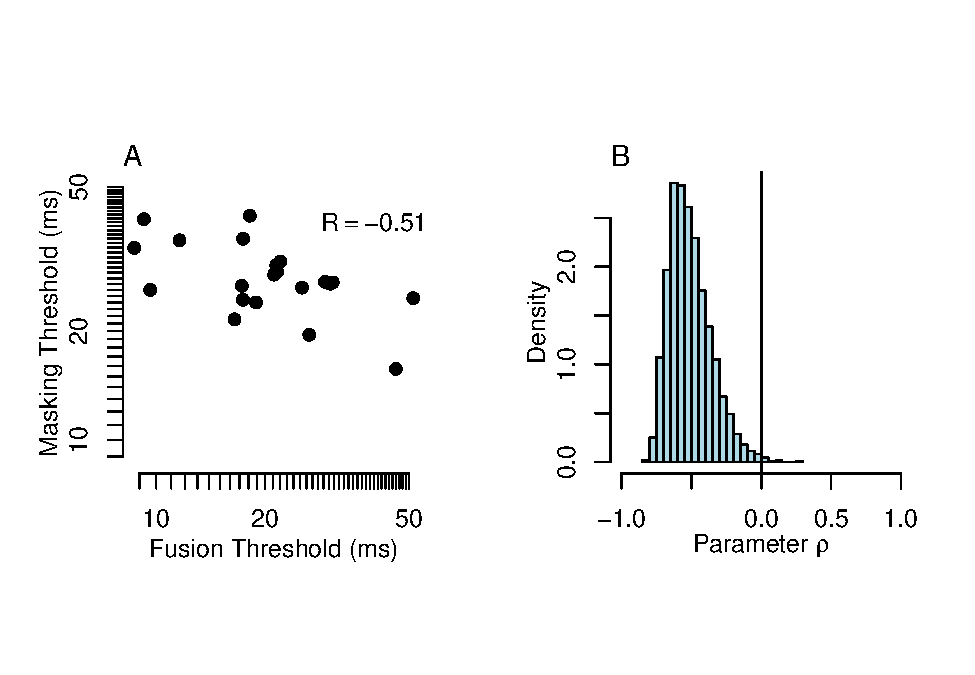
\includegraphics{p_files/figure-latex/results-1} \caption{A. Scatter plot of thresholds show a negative correlation across tasks.  B. Posterior distribution of correlation coefficient $\rho$ shows decisive evidence for a negative correlation.}\label{fig:results}
\end{figure}

The statistical significance of the results was assessed through Bayes factor as follows: Let \(T_{ij}\) denote the log-threshold for the \(i\)th individual in the \(j\)th task, \(j=1,2\) for the masking and fusion tasks, respectively. These thresholds are scaled into \(z\)-scores: \(Z_{ij}=(T_{ij}-m_j)/s_j,\) where \(m_j\) and \(s_j\) are the mean and standard deviation of these thresholds for each task. These z-scores are modeled as:
\[
\begin{pmatrix} Z_{i1}\\ Z_{i2} \end{pmatrix} \mid \rho \sim \mbox{N}_2\left[
\begin{pmatrix} 0 \\ 0 \\ \end{pmatrix}, \;
\begin{pmatrix} 1 & \rho\\ \rho & 1\end{pmatrix}
\right]
\]
where \(\rho\) is the population correlation among the two tasks. The model is conditional on \(\rho\) which, in turn, must be specified. A general model without a sign constraint on correlation, denoted \(\calM_g\), is:
\[
\calM_g: \quad \rho \sim \mbox{Unif}(-1,1).
\]
The two competing hypotheses are expressed as sign constraints:

\[\begin{aligned}
\calM_-:& \quad \rho \sim \mbox{Unif}(-1,0)\\
\calM_+:& \quad \rho \sim \mbox{Unif}(0,1)
\end{aligned}
\]

The main target of inference is the Bayes factor between \(\calM_-\) and \(\calM_+\). The Bayes factor is the probability of the data under one model relative to the other:
\[
B_{-,+}\;=\;\frac{\Pr(\bfZ \mid \calM_-)}{\Pr(\bfZ \mid \calM_+)},
\]
where \(\bfZ\) is the collection of all \(z\)-scored thresholds. Computation of the Bayes factor is convenient in the encompassing approach (Hoijtink, Klugkist, \& Boelen, 2008). Accordingly,
\begin{equation} \label{BF}
B_{-,+}\;=\;\frac{\Pr(\bfZ \mid \calM_-)}{\Pr(\bfZ \mid \calM_+)} = \frac{\Pr(\rho<0|\bfZ, \calM_g)}{\Pr(\rho>0|\bfZ,\calM_g)}.
\end{equation}
According to (\ref{BF}), the critical quantity is the posterior distribution of parameter \(\rho\) under the general model. The Bayes factor is a ratio of how much probability mass of this posterior is below zero relative to how much is above zero. In analysis, this posterior distribution may be sampled in JAGS (Plummer, 2003) or stan (Carpenter et al., 2017), and the proportions of samples above and below zero serves as the probability mass.

Figure \ref{fig:results}B shows the posterior distribution of \(\rho\) under the general model. The posterior mean is -0.51;
the amount of mass below and above zero is 0.9961 and 0.0039, respectively, and the corresponding Bayes factor is 256 in favor of the negative model. This ratio is decisive: thresholds are negatively correlated and performance is positively correlated.

Note that the comparison here is different from the usual one where we wish to compare zero or null correlation to some correlation, be it positive or negative. Here, we explicitly use the positive-vs-negative comparison because it maps exactly into the competing hypotheses. The usage of Bayes factors allow researchers the flexibility to test the propositions of greatest theoretical interest rather than the one-size-fits-all approach inherent in null-hypothesis significance testing (Rouder, Morey, \& Wagenmakers, 2016).

The analysis here is predicated on an opposing role of duration. In designing the staircases, we assumed that long durations negatively and positively affected accuracy in masking and fusion, respectively. Is it so?
Figure \ref{fig:result2} shows the effect of duration on accuracy. To make data from individuals comparable, duration was measured as a multiple of individual's threshold. The many points on the figure come about because each individual experiences several different levels of duration, and there is a point for each individual-by-duration combination. The lines are loess smooths (Cleveland, 1981), and the trends are obvious and in the expected direction. Indeed, duration plays an opposing role in the tasks.

\begin{figure}[h]
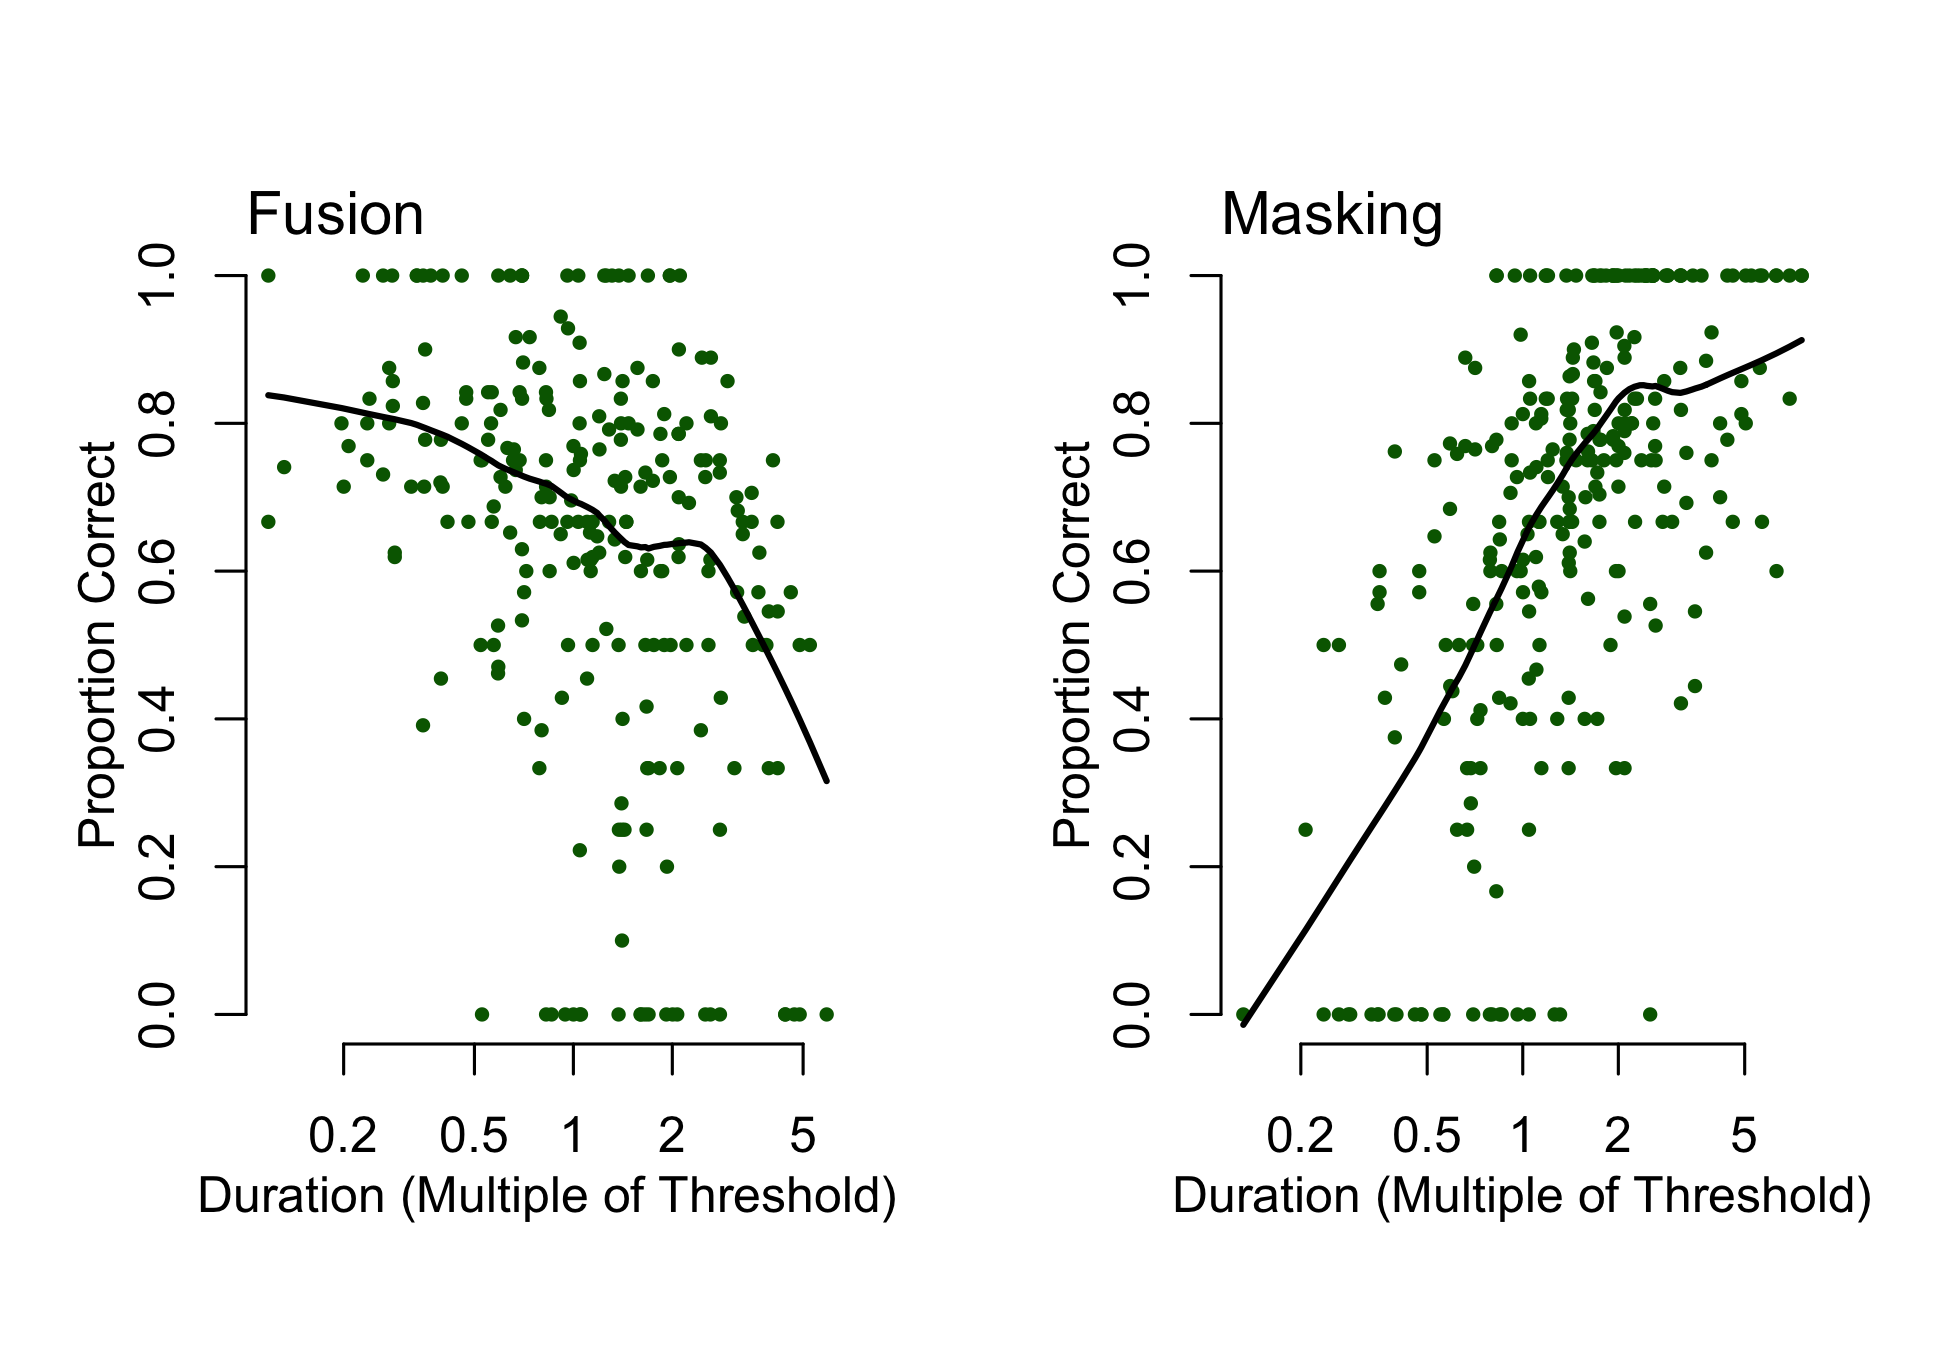
\includegraphics{p_files/figure-latex/result2-1} \caption{Duration plays an opposite role in fusion and masking.  Increasing duration negatively affects fusion performance and positively affects masking performance.  Points are individual-by-duration-level combinations.}\label{fig:result2}
\end{figure}

\hypertarget{discussion}{%
\section{Discussion}\label{discussion}}

A common theme in vision theories is that there is a small temporal window of integration. We asked whether variation in the duration of this window is a driver of individual differences in fusion and masking tasks. If this variation was a driver, one would expect a novel negative correlation where people with longer windows perform better at the fusion task and worse at the masking task. This negative correlation did not hold. People who performed better in the masking task also performed better at the fusion task. This pattern cannot be accounted for with variation in the temporal window.

What type of mechanisms could account for these individual-difference patterns? An alternative account for backwards masking is an \emph{interruption} account (Kahneman, 1968). Accordingly, it takes time to process the target, and the presentation of the mask interrupts this processing. Target processing is terminated before the target is registered and processing of the mask proceeds unabated. The conventional means of discriminating between an integration account and an interruption account is to vary both the brightness and timing of the target and mask. The integration account predicts that the relative integrated energy or brightness determines performance; the interruption account predicts that the ISI determines performance. By-and-large, many researchers ascribe that both integration accounts and interruption accounts hold, but for different stimuli, at different time scales, and at different levels of the visual system (Enns \& Di Lollo, 2000; Turvey, 1973). To rough approximation, integration seems to hold at more sensory levels, on time scales less than 100 ms, for low-contrast targets, and for masks that are either pedestals or fine-grained white noise. Interruption seems to be at a more central level, on time scales around 200 ms, for well-contrasted targets that are objects and masks that have object features. Moreover, integration is more compatible with forward masking (the deleterious effect of a mask preceding a target) and interruption is more compatible with backwards masking, metacontrast masking (Bridgeman, 1971) and object-substitution masking (Enns \& Di Lollo, 2007). We suspect that our target and mask are object-like in that they have well localized positions, and that interruption may be more responsible for masking than integration.

If interruption is the main source of masking in this task, then the speed of readout from iconic memory may vary across people. But what does this speed have to do with the fusion task? We suspect that the fusion task too is not a matter of simple energy integration. Instead, the rapidly presented first target needs to be actively maintained in iconic memory during the ISI. We speculate that there is a refreshing processes (Camos et al., 2018), and the speed of refreshing may determine the success of maintenance. The positive correlation may come about from a common facility in reading from and maintaining iconic memory.

Of course, the positive correlation found here in performance may have a more mundane source such as motivation. While we cannot rule such factors out, we think some obvious sources of motivation differences may be ruled out by the design. People who do poorly or feel they do poorly on tasks are not well motivated. One worries about motivation differences when people who do well are more rewarded. Yet, here, because of the adaptive design, all participants had the same level of performance and received positive feedback on about 71\% of trials. Participants had no notion of how fast the stimuli were flashed, and certainly had no basis to compare their performance to others.

The main message here is that the temporal window of integration does not account for individual differences and that theories of what may do so remain speculative for now.

\newpage

\hypertarget{references}{%
\section*{References}\label{references}}
\addcontentsline{toc}{section}{References}

\hypertarget{refs}{}
\begin{CSLReferences}{1}{0}
\leavevmode\vadjust pre{\hypertarget{ref-Allport.1968}{}}%
Allport, D. A. (1968). Phenomenal simultaneity and the percpetual moment hypothesis. \emph{British Journal of Psychology}, \emph{59}(4), 395--406. doi:\href{https://doi.org/10.1111/j.2044-8295.1968.tb01154.x}{10.1111/j.2044-8295.1968.tb01154.x}

\leavevmode\vadjust pre{\hypertarget{ref-Breitmeyer.1984}{}}%
Breitmeyer, B. G. (1984). \emph{Visual {Masking}: {An} integrative approach}. New York: Oxford University Press.

\leavevmode\vadjust pre{\hypertarget{ref-Bridgeman.1971}{}}%
Bridgeman, B. (1971). Metacontrast and lateral inhibition. \emph{Psychological Review}, \emph{78}(6), 528--539. doi:\href{https://doi.org/10.1037/h0031782}{10.1037/h0031782}

\leavevmode\vadjust pre{\hypertarget{ref-Busey.Loftus.1994}{}}%
Busey, T. A., \& Loftus, G. R. (1994). Sensory and cognitive components of visual information acquisition. \emph{Psychological Review}, \emph{101}, 446--469.

\leavevmode\vadjust pre{\hypertarget{ref-Camos.etal.2018}{}}%
Camos, V., Johnson, M., Loaiza, V., Portrat, S., Souza, A., \& Vergauwe, E. (2018). What is attentional refreshing in working memory? \emph{Annals of the New York Academy of Sciences}, \emph{1424}(1), 19--32. doi:\href{https://doi.org/10.1111/nyas.13616}{10.1111/nyas.13616}

\leavevmode\vadjust pre{\hypertarget{ref-Carpenter.etal.2017}{}}%
Carpenter, B., Gelman, A., Hoffman, M. D., Lee, D., Goodrich, B., Bettencourt, M., \ldots{} Riddell, A. (2017). Stan: {A} probabilistic programming language. \emph{Journal of Statistical Software}, \emph{76}.

\leavevmode\vadjust pre{\hypertarget{ref-Cleveland.1981}{}}%
Cleveland, W. S. (1981). {LOWESS}: {A} program for smoothing scatterplots by robust locally weighted regression. \emph{The American Statistician}, \emph{35}, 54.

\leavevmode\vadjust pre{\hypertarget{ref-DiLollo.1980}{}}%
Di Lollo, V. (1980). Temporal integration in visual memory. \emph{Journal of Experimental Psychology: General}, \emph{109}(1), 75. Retrieved from \url{https://psycnet.apa.org/journals/xge/109/1/75/}

\leavevmode\vadjust pre{\hypertarget{ref-DiLollo.Wilson.1978}{}}%
Di Lollo, V., \& Wilson, A. E. (1978). Iconic persistence and perceptual moment as determinants of temporal integration in vision. \emph{Vision Research}, \emph{18}(12), 1607--1610. Retrieved from \url{https://www.sciencedirect.com/science/article/pii/0042698978902511}

\leavevmode\vadjust pre{\hypertarget{ref-Enns.DiLollo.2000}{}}%
Enns, J. T., \& Di Lollo, V. (2000). What's new in visual masking? \emph{Trends in Cognitive Sciences}, \emph{4}(9), 345--352. Retrieved from \url{https://www.cell.com/AJHG/fulltext/S1364-6613(00)01520-5}

\leavevmode\vadjust pre{\hypertarget{ref-Enns.DiLollo.2007}{}}%
Enns, J. T., \& Di Lollo, V. (2007). Object substitution: {A} new form of visual masking in unattended visual locations. \emph{Psychological Science}, \emph{8}, 135--139.

\leavevmode\vadjust pre{\hypertarget{ref-Hoijtink.etal.2008}{}}%
Hoijtink, H., Klugkist, I., \& Boelen, P. (2008). \emph{Bayesian evaluation of informative hypotheses}. New York: Springer.

\leavevmode\vadjust pre{\hypertarget{ref-Kahneman.1968}{}}%
Kahneman, D. (1968). Method, findings, and theory in studies of visual masking. \emph{Psychological Bulletin}, \emph{70}, 404--425. doi:\href{https://doi.org/10.1037/h0026731}{10.1037/h0026731}

\leavevmode\vadjust pre{\hypertarget{ref-Levitt.1971}{}}%
Levitt, H. (1971). Transformed {Up}‐{Down Methods} in {Psychoacoustics}. \emph{The Journal of the Acoustical Society of America}, \emph{49}, 467--477. doi:\href{https://doi.org/10.1121/1.1912375}{10.1121/1.1912375}

\leavevmode\vadjust pre{\hypertarget{ref-Plummer.2003}{}}%
Plummer, M. (2003). {JAGS}: {A Program} for {Analysis} of {Bayesian Graphical Models Using Gibbs Sampling}. In \emph{Proceedings of the 3rd {International Workshop} on {Distributed Statistical Computing}}.

\leavevmode\vadjust pre{\hypertarget{ref-Ritchie.2015}{}}%
Ritchie, S. (2015). \emph{Intelligence: {All} that matters}. John Murray. Retrieved from \url{https://books.google.com/books?hl=en\&lr=\&id=aO7rBQAAQBAJ\&oi=fnd\&pg=PT5\&dq=stuart+ritchie+intelligence\&ots=qBxxyI-OP0\&sig=oqO-M6CAezJXDYDoVkbq2MEOAkE}

\leavevmode\vadjust pre{\hypertarget{ref-Rouder.etal.2016c}{}}%
Rouder, J. N., Morey, R. D., \& Wagenmakers, E.-J. (2016). The {Interplay} between {Subjectivity}, {Statistical Practice}, and {Psychological Science}. \emph{Collabra}, \emph{2}, 6. Retrieved from \url{http://doi.org/10.1525/collabra.28}

\leavevmode\vadjust pre{\hypertarget{ref-Scharnowski.etal.2007}{}}%
Scharnowski, F., Hermens, F., \& Herzog, M. H. (2007). Bloch's law and the dynamics of feature fusion. \emph{Vision Research}, \emph{47}(18), 2444--2452. doi:\href{https://doi.org/10.1016/j.visres.2007.05.004}{10.1016/j.visres.2007.05.004}

\leavevmode\vadjust pre{\hypertarget{ref-Schonbrodt.etal.2017}{}}%
Schönbrodt, F. D., Wagenmakers, E.-J., Zehetleitner, M., \& Perugini, M. (2017). Sequential hypothesis testing with {Bayes} factors: {Efficiently} testing mean differences. \emph{Psychological Methods}, \emph{22}(2), 322--339.

\leavevmode\vadjust pre{\hypertarget{ref-Smith.1995}{}}%
Smith, P. L. (1995). Multiple detector models of visual simple reaction time. \emph{Psychological Review}, \emph{102}, 567--593.

\leavevmode\vadjust pre{\hypertarget{ref-Stroud.1956}{}}%
Stroud, J. M. (1956). The fine structure of psychological time. Retrieved from \url{https://psycnet.apa.org/record/1957-02922-010}

\leavevmode\vadjust pre{\hypertarget{ref-Turvey.1973}{}}%
Turvey, M. T. (1973). On peripheral and central processes in vision: {Inferences} from an information-processing analysis of masking with patterned stimuli. \emph{Psychological Review}, \emph{80}, 1--52.

\end{CSLReferences}


\end{document}
